\documentclass[12pt,a4paper]{article}

%\usepackage[left=2cm, right=2cm, top=4cm, bottom=2cm]{geometry}
\usepackage[utf8]{inputenc}
\usepackage[spanish]{babel}
\usepackage{enumitem}
\usepackage{amsmath}
\usepackage{tikz}

\usepackage{hyperref}
\hypersetup{
    colorlinks=true,
    linkcolor=blue,
    filecolor=magenta,
    urlcolor=cyan,
}


\bibliographystyle{alpha}
\bibliography{bibfile}

\begin{document}

\begin{titlepage}
	\centering
	{\scshape\LARGE Universidad Nacional Autónoma de México \par}
	\vspace{1cm}
	{\scshape\Large Computación Distribuida\par}
	\vspace{1cm}
	{\huge\bfseries Algoritmos Autorregulables\par}
	\vspace{1cm}
    {\Large\itshape Jerónimo Almeida Rodríguez \par}
    \vspace{.5cm}
	{\Large\itshape Edgar Quiroz Castañeda \par}
    \vspace{.5cm}
	{\Large\itshape Naomi Reyes ...\par}
	\vfill
	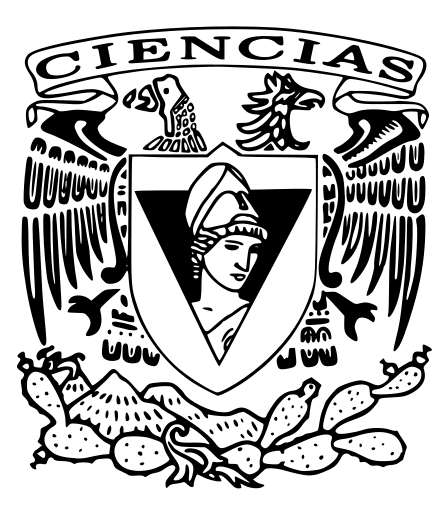
\includegraphics[width=0.5\textwidth]{escudo_f-ciencias.png}
	\vfill

	{\large Viernes 14 de Diciembre del 2018 \par}
\end{titlepage}

	\pagebreak
	\setlength{\voffset}{-0.75in}
	\setlength{\headsep}{5pt}


\begin{center}
		\textsc{\huge Algoritmos Autorregulables\\}
		\textit{Jerónimo Almeida, Edgar Quiroz, Naomi Reyes\\}
        14/12/2018
\end{center}

Los algoritmos Autorregulables son aquellos que, después de definido un estado
válido, todos los procesos que ejecuten dicho algoritmo tienden después de
algún tiempo a alcanzarlo sin importar el estado actual en el que se encuentren,
es decir, que pueden iniciar en cualquier estado arbitrario no válido o después
de que haya ocurrido algún error, el proceso llegue a un estado válido .



\section{Introducción}{
\subsection{Motivación}{
    Que el sistema se recupere de un error sin intervención humana, es decir que
    dado un estado global arbitrario (particularmente erróneo), dar un algoritmo
    que haga que el estado global eventualmente se vuelva válido.
}
\subsection{Especificación}{
    Texto de relleno
}
\subsection{Modelo}{}
}
\section{Pase de Token en un Anillo}{}
\section{Sincronizadores}{
\subsection{Generalidades de sincronizadores}{}

\subsection{Sincronizador $\alpha$}{}

\subsection{Sincronizador autorregulable}{}

    \subsubsection{Regla Simple}{}

    \subsubsection{Segunda Regla}{}

    \subsubsection{Regla Óptima}{}
}
\section{Conclusión}{}

\begin{thebibliography}{}

\bibitem[Asp18]{Asp18}
James Aspnes. Notes on Theory of Distributed Systems.
\href{http://www.cs.yale.edu/homes/aspnes/classes/465/notes.pdf}
{http://www.cs.yale.edu/homes/aspnes/classes/465/notes.pdf}, October 2018.

\end{thebibliography}
\end{document}
